\section{Circular buffer API}
\label{sec:circ-api}

The circular buffer is a fixed-size, \emph{on-disk} queue of
updates, which are pairs of an address and a disk block. It is used to implement
write-ahead logging: updates are first stored in the circular buffer, and
then eventually moved to a separate data region. It supports two operations
during normal usage: \cc{Append(end, upds)} appends a list of updates to the buffer
and \cc{TrimTill(pos)} deletes updates up to the position \cc{pos}. These logical queue positions grow
indefinitely, but the buffer can hold a finite and fixed number of update at a time and it
is the caller's responsibility to avoid overflowing with \cc{Append}. The only
read operation is recovery, which restores the durable updates and current queue
position; the write-ahead log caches updates during normal execution, but this
is not the circular buffer's concern. The complete Go API is shown in
\cref{fig:circ:api}.

\begin{figure}[ht]
\begin{minted}{go}
// Circular buffer Go API

func InitCircular() *Appender
func (c *Appender) Append(end uint64, upds []Update)
func TrimTill(start uint64)
func RecoverCircular() (c *Appender, start uint64, upds []Update)

type Update {
  Addr  uint64
  Block []byte
}
\end{minted}
  \caption{The Go API for the circular buffer.}%
  \label{fig:circ:api}
\end{figure}

\begin{figure}[ht]
  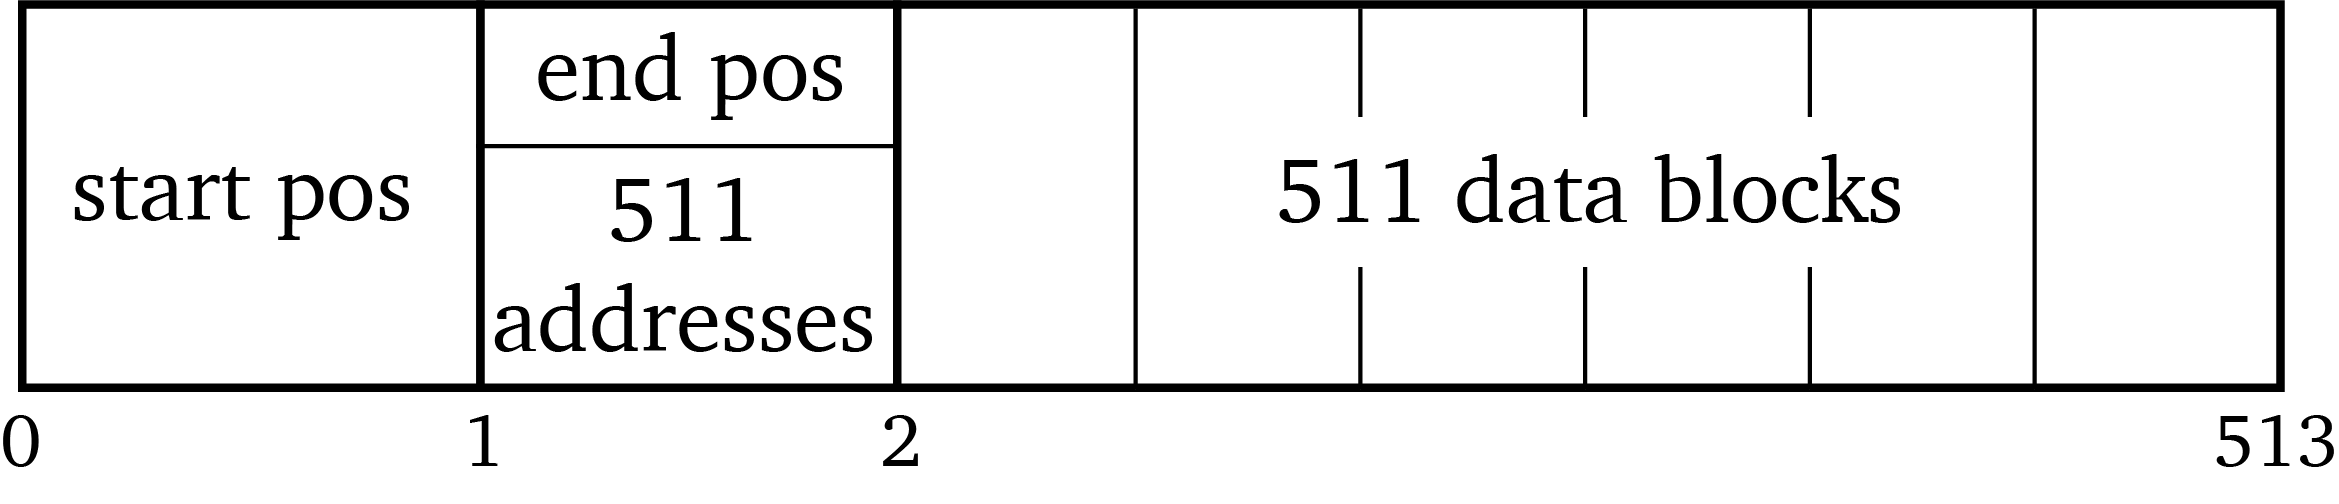
\includegraphics{fig/circ-phys.png}
  \caption[Circular buffer on-disk layout]%
  {The circular buffer's on-disk layout, consisting of a fixed 513 blocks
  located at the beginning of the disk.}
\label{fig:circ:phys}
\end{figure}

The basic idea is that the circular buffer is specified in terms of an abstract
state that transitions for each operation. The recovery operation
restores the pre-crash state of the queue from disk. The state for this library consists
of two components: a queue of updates (which are pairs of an address to write to
and a 4KB block to write there) and a 64-bit start position that indicates how
many updates occurred prior to the current list of updates. The \cc{Append} operation, as
mentioned, simply appends to the list of updates. The argument to \cc{TrimTill}
is an absolute position; the effect of \cc{TrimTill(pos)} is to delete
\cc{pos - start} updates from the beginning of the list of updates and set the
new start position to \cc{pos}. A more formal specification is given in
\cref{fig:circ:spec}.

The circular buffer supports atomic and concurrent \cc{Append} and \cc{TrimTill}
with a careful on-disk layout. It consists of two header blocks and 511 data
blocks, depicted graphically in \cref{fig:circ:phys}. The first header block
(the ``trim'' block, since it is used for trimming) holds the logical start
position of the queue, while the second header (the ``append'' block, since it
is used for appending) holds the logical end position and 511 addresses; the
data blocks for these addresses are in the remaining data blocks. This append
header has 4096 bytes, or enough space for 512 64-bit numbers; one is used for
the end position, and the remainder for update addresses. Recovery uses the
header blocks to determine what subset of the circular buffer holds complete
multiwrites; partially-appended updates are ignored for atomicity.

To append atomically, \cc{c.Append(end, upds)} first writes the data (using
\cc{end} to know where to start writing), and then writes the append header
block to atomically incorporate the writes, and simultaneously to write the
addresses. The in-memory \cc{c *Appender} struct keeps track of the existing
addresses so they can be re-written to disk. Meanwhile \cc{TrimTill} logically
deletes by merely writing a new, higher start position to the trim header.

Since these operations touch disjoint parts of disk, they can be performed
concurrently. However, one subtlety is that it is important to preserve the
queue abstraction that append operations do not overflow the circular buffer
(since this would overwrite old values) and that trim operations do not delete
past the current end (this would invalidate future appends immediately). The
insight that allows the caller to guarantee these properties is that the start
and end positions of the circular buffer are monotonically increasing, meaning
any snapshot of their positions is a \emph{lower bound} that is valid from then
on. Thus without holding any locks a call to \cc{c.TrimTill(newStart)} can
guarantee that the trim fits by showing that $\cc{newStart} \leq \cc{end_lb}$,
where \cc{end_lb} is merely a lower bound and not necessarily the exact end
position. However, it is necessary for the caller to know the exact start
position and that it will not change concurrently, in order to guarantee that
\cc{newStart} is greater than the current \cc{start}. The proof of
\cc{c.Append(end, upds)} is the dual of trim, requiring a lower bound on the
start position and exact control over \cc{end}.

\begin{figure}[ht]
\begin{minted}{coq}
(* Circular buffer Coq specification *)

Definition update := u64 * Block;
Record circ_state := {
  upds: list update;
  start: u64;
}.

(* requires length s.(upds) + length new_upds <= 511 *)
Definition append (s: circ_state) (new_upds: list update) : circ_state :=
  s <[ upds := s.(upds) ++ new_upds ]>.

(* requires s.(start) <= new_start *)
Definition trim_till (s: circ_state) (new_start: u64) : circ_state :=
  let num_removed := new_start - s.(start) in
  s <[ start := new_start ]>
    <[ upds := drop num_removed s.(upds) ]>.
\end{minted}
  \caption{The specification for the circular buffer, described as transitions
    on the abstract state.}
  \label{fig:circ:spec}
\end{figure}


There are three challenges in specifying how the circular buffer's
implementation connects to the abstract transitions given above. First, we
want to show that \cc{Append} appears to be atomic to the caller, even though
its implementation writes many disk blocks and the system could crash after
persisting only some of them. Second, the library has some thread-safety
requirements to enforce on the caller: in particular \cc{Append} and
\cc{TrimTill} can be called concurrently from separate threads, but it is not
safe to concurrently issue multiple appends or multiple trim requests. Finally, the library
relies on the caller to guarantee that \cc{Append} and \cc{TrimTill} are called with enough
available space. These last two challenges are due to leaving concurrency
control to the caller, which is more efficient than the circular buffer having
its own redundant locking.

The write-ahead log uses the circular buffer from two threads, one dedicated to
\emph{logging} which appends to the circular buffer to make writes durable and another
dedicated to \emph{installation} which trims writes from the circular buffer
after installing them. Appending and trimming can be performed concurrently, but
appending requires the \cc{*Appender} struct which is not thread-safe. The
caller only reads from the circular buffer if the system crashes, at which point
recovery restores the previous state.

\section{Circular buffer custom resources}

Perennial, like Iris, has support for user-defined separation-logic resources.
These are defined using lower-level mechanisms, but this section simply presents the
resources and the intuition for how they are used without going into details on
how they are implemented. The circular buffer defines and issues the
following custom separation-logic resources:

\newidentmacro{length}
\newcommand{\circstate}{\cc{circ_state}}
\newcommand{\startIs}{\cc{start_is}}
\newcommand{\diskendIs}{\cc{end_is}}

\begin{itemize}
  \item $\circstate(\gamma, \sigma)$, which says that the current state
  of the circular buffer is $\sigma$. The $\gamma$ argument is a ``ghost name''
  for the ghost state associated with this instance of the circular buffer; at
  any time there is only one circular buffer, but this name will change every
  time the system crashes and reboots and thus distinguishes different
  ``generations'' of the circular buffer.
  \item $\cc{is_circular}(\gamma)$, defined to be the invariant assertion
  $\knowInv{}{\exists \sigma, \circstate(\gamma, \sigma) * P(\sigma)}$.
  The $P(\sigma)$ part of this invariant is part of the HOCAP specification
  style, explained below.
  \item $\cc{circ_appender}(\gamma, \ell)$. This relates the circular buffer's
  ghost state with $\ell$, a \cc{*circularAppender} pointer that has some data
  needed to append to the circular buffer. This resource is not persistent and
  is owned by the logger thread.
  \item $\startIs(\gamma, \cc{start})$ and
  $\diskendIs(\gamma, \cc{end})$ give the exact current positions of the start
  and end (that is, $\sigma.\cc{start} + \length(\sigma.\cc{updates})$) of
  the circular buffer. These resources are not persistent and are owned by
  the installer and logger threads respectively.
  \item $\cc{start_at_least}(\gamma, \cc{start})$ and
  $\cc{end_at_least}(\gamma, \cc{end})$ give \emph{lower bounds} on the start
  and end positions. It is possible to issue such resources because the start and
  end monotonically increase. As a result of monotonicity, these resources are
  persistent; once \cc{start} or \cc{end} reaches some value, that value is
  always a valid lower bound.
\end{itemize}

\section[Specifications for Append and TrimTill]%
{Specifications for \cc{Append} and \cc{TrimTill}}

Formally the way each operation is specified is using a style called
higher-order concurrent abstract predicates (HOCAP)~\cite{svendsen:hocap,jacobs:logatom}. The basic idea is that the
library maintains an invariant $P(\sigma)$, where $\sigma$ is the current
abstract state; a key idea in the HOCAP specification is that this predicate $P$
is chosen by \emph{the client} (that is, the code calling the library).

The predicates in HOCAP specifications express ownership over ghost state. This
aspect of Perennial is inherited from Iris and described in more detail in
\cref{sec:perennial:concurrency}. In this chapter we use the \emph{view-shift
assertion} $R \vs Q$ to express ghost updates, which are used to update the
predicate $P(\sigma)$ that the library maintains.\footnote{Note that this is a slight
change in notation, compared to the update modality used in the Perennial chapter; the view shift is equivalent to
$R \wand \upd Q$.} The intuition for $R \vs Q$ is that it represents some
resources which allow the holder of the assertion to take
$R \sep (R \vs Q)$ and ``fire'' the view shift, updating the underlying ghost
variables, and finally obtain $Q$.

For each operation, the client passes in a
view-shift $P(\sigma) \vs P(\sigma') * Q$, for any
transition from $\sigma$ to $\sigma'$ that is a valid transition for the operation.
This view shift represents a kind of once-usable ``callback'' which transforms
$P(\sigma)$ into $P(\sigma')$, by updating the caller's ghost state in
$P$. At the end of the operation, the client receives $Q$ as a kind of
certificate that the callback ran. The intuition here is that the library's proof must
``fire'' or ``call'' the view shift in order to preserve $P$ and produce $Q$,
but the proof gets to pick the exact moment when it should fire the view shift,
which is the linearization point of the operation. Note that the view shift
might be proven using exclusive resources that cannot be duplicated, so it is
important that it is only fired once.

We can see both the HOCAP pattern and the circular-buffer resources in action in
the specification for Append:
%
\begin{align*}
  &\{ \cc{is_circular}(\gamma) \sep {} \\
&\quad (\forall \sigma, P(\sigma) \vs P(\sigma \lappend \cc{upds}) * Q) \sep {} \\
&\quad \cc{circ_appender}(\gamma, \cc{c}) \sep {} \\
&\quad \diskendIs(\cc{end}) \sep \cc{start_at_least}(\cc{start}) \sep (\cc{end} - \cc{start} + \length(\cc{upds}) \leq 511) \\
&\} \\
&\qquad\cc{c.Append(end, upds)} \\
&\{ \cc{circ_appender}(\gamma, \cc{c}) \sep {} \\
&\quad \diskendIs(\cc{end} + \length(\cc{upds})) \sep Q \}
\end{align*}

There are several aspects to the specification, mostly in the precondition. The
first line is the most straightforward: we need the circular buffer's invariant
to hold, for a particular ghost name $\gamma$. The second line is part of the
general HOCAP pattern. The view shift updates $P(\sigma)$ to the appropriate new
state, denoted with $\sigma \lappend \cc{upds}$ as shorthand for $\sigma$ with \cc{upds}
appended to the updates field (and the same \cc{start}). The proof of this
specification executes the view shift at the linearization point of the \cc{Append}
operation, changing the state inside the $\cc{is_circular}$ invariant. The view
shift produces a client-supplied assertion $Q$, which is returned in the
postcondition.

The assertion $\cc{circ_appender}(\gamma, \cc{c})$ asserts that the
in-memory state cached in \cc{c} is correct (these are the addresses for the
updates but not their contents). This resource is unique, since the appending
thread needs ownership this in-memory buffer, and is returned in the
postcondition for the next \cc{Append} operation. Exclusive ownership over this
buffer is one reason why appending is only safe from one thread.

The rest of the specification is specific to how the circular buffer manages
concurrency. Appending requires precise knowledge of the end position of the
circular buffer, which the logger thread maintains. A lower bound on the start
position is sufficient to prove that there is currently---and will continue to
be---enough space for the updates to fit on disk; the left-hand side of the
inequality computes an \emph{upper bound} on how much space will be used after
the append because the \cc{start} variable is a lower bound. The postcondition
gives the caller back the $\diskendIs$ assertion with the new precise end point.
Note that the precondition guarantees that the append will not fail due to
running out of space. Because the start and end are manipulated without locks
the circular buffer implementation does not even have a way to safely
dynamically check if there is enough space.

The specification for \cc{TrimTill} is similar to Append:
%
\begin{align*}
  &\{ \cc{is_circular}(\gamma) \sep {} \\
&\quad (\forall \sigma, P(\sigma) \vs P(\sigma[:\cc{newStart}]) * Q) \sep {} \\
&\quad \startIs(\cc{start}) \sep \cc{end_at_least}(\cc{end}) \sep (\cc{start} \leq \cc{newStart} \leq \cc{end}) \\
&\} \\
&\qquad\cc{c.TrimTill(newStart)} \\
&\{ \startIs(\cc{newStart}) \sep Q \}
\end{align*}

The effect of a \cc{TrimTill}, abbreviated $\sigma[:\cc{newStart}]$, is to set
the start position and delete the first $\cc{newStart} - \cc{start}$ updates.
For this operation to be safe, it requires
that the start not go backwards (recall the Append proof relies on a lower bound
for \cc{start}) and not go past the current end position (concretely this would
logically delete updates that haven't yet been written!). The precondition
encodes these by taking a precise current \cc{start} position and a lower bound
on the end, and then requiring the new start variable be between the two. Just
like with Append, the installer thread that calls this operation always
maintains precise knowledge (ownership) of the start of the circular buffer.

Notice that neither of these specifications have a crash condition. The reason
this is not required is because both methods already maintain an Iris invariant in
the \cc{is_circular} predicate. The next
section,~\ref{sec:perennial:recovery-spec}, details how crashes and recovery are
specified in Perennial.
